\def\SECTION{1.3 Midpoint \& Distance}
\documentclass[aspectratio=169,14pt]{beamer}
\usepackage[T1]{fontenc}
\usepackage{mathpazo}
\usepackage{amsmath,amssymb}
\usepackage{tikz}
\usetikzlibrary{arrows.meta,calc,decorations.pathreplacing}
\definecolor{fblue}{HTML}{1F4E79}
\definecolor{fteal}{HTML}{0F7C7C}
\definecolor{fgold}{HTML}{C9962B}
\definecolor{fred}{HTML}{B3261E}
\definecolor{fink}{HTML}{16233B}
\definecolor{fsoft}{HTML}{EEF3F8}
\definecolor{fgoldsoft}{HTML}{FBF1DC}
\setbeamertemplate{navigation symbols}{}
\setbeamercolor{normal text}{fg=fink}
\setbeamercolor{frametitle}{fg=fblue}
\setbeamerfont{frametitle}{series=\bfseries,size=\Large}
\setbeamercolor{structure}{fg=fteal}
\setbeamertemplate{itemize item}{\color{fteal}$\blacktriangleright$}
\setbeamertemplate{frametitle}{\vspace{6pt}\insertframetitle\par\vspace{-2pt}{\color{fgold}\rule{2.2cm}{2pt}}}
\setbeamertemplate{footline}{\hspace{0.6cm}{\color{fblue}\scriptsize\bfseries Prof.\ Fang \textcolor{fteal}{Math}}\hfill{\scriptsize\color{gray}\SECTION\quad\insertframenumber}\hspace{0.6cm}\vspace{6pt}}
\newcommand{\key}[1]{{\color{fteal}\textbf{#1}}}
\newcommand{\ans}[1]{\colorbox{fgoldsoft}{\color{fink}\ensuremath{#1}}}
\newcommand{\warn}[1]{\begin{beamercolorbox}[sep=8pt,rounded=true]{warnbox}{\color{fred}\textbf{Watch out!}}\enskip #1\end{beamercolorbox}}
\setbeamercolor{warnbox}{bg=fred!8,fg=fink}
\setbeamercolor{turnbox}{bg=fgoldsoft,fg=fink}
\setbeamercolor{defbox}{bg=fsoft,fg=fink}
\newcommand{\defn}[1]{\begin{beamercolorbox}[sep=8pt,rounded=true]{defbox}#1\end{beamercolorbox}}
\newenvironment{yourturn}{\begin{beamercolorbox}[sep=10pt,rounded=true]{turnbox}{\color{fgold}\Large\bfseries Your turn!}\quad{\small Pause the video and try it.}\par\medskip}{\end{beamercolorbox}}
\newcommand{\titleframe}[3]{%
\begin{frame}[plain]
\begin{tikzpicture}[remember picture,overlay]
\fill[fblue] (current page.north west) rectangle ([yshift=-0.9cm]current page.north east);
\node[anchor=west,text=white,font=\bfseries] at ([xshift=0.6cm,yshift=-0.45cm]current page.north west) {Prof.\ Fang \textcolor{fgold}{Math}};
\node[anchor=east,text=white,font=\small] at ([xshift=-0.6cm,yshift=-0.45cm]current page.north east) {Geometry $\cdot$ Chapter 1};
\end{tikzpicture}
\vfill
{\color{fteal}\large\bfseries #1}\par\medskip
{\color{fblue}\fontsize{30}{34}\selectfont\bfseries #2}\par\medskip
{\color{fgold}\rule{3cm}{3pt}}\par\bigskip
{\large #3}
\vfill
{\small\color{gray} fangmath.com $\cdot$ YouTube @3SMath}
\end{frame}}
\newcommand{\closeframe}[1]{%
\begin{frame}{Remember}
#1
\vfill
\begin{center}{\color{fblue}\large\bfseries Now practice at your level:}\par\smallskip
{\Large\color{fteal}\bfseries fangmath.com} \enskip{\color{gray}$\to$ Geometry $\to$ Chapter 1}\end{center}
\end{frame}}

\usepackage{pgfplots}\pgfplotsset{compat=1.17}
\newcommand{\grid}[4]{\draw[step=1,gray!25] (#1,#2) grid (#3,#4);\draw[-{Stealth},gray] (#1,0)--(#3+0.3,0) node[right]{\small$x$};\draw[-{Stealth},gray] (0,#2)--(0,#4+0.3) node[above]{\small$y$};}
\begin{document}
\titleframe{Lesson 1.3}{Midpoint \& Distance Formula}{Two formulas --- and how to never mix them up}

\begin{frame}{The trick}
\vfill
\centering
{\fontsize{34}{40}\selectfont\color{fteal}\textbf{M}\color{fink}idpoint $=$ \color{fteal}\textbf{M}\color{fink}ean}\par\bigskip\pause
{\fontsize{34}{40}\selectfont\color{fgold}\textbf{D}\color{fink}istance $=$ \color{fgold}\textbf{D}\color{fink}ifference}
\vfill
\end{frame}

\begin{frame}{Midpoint: simple case first}
\centering
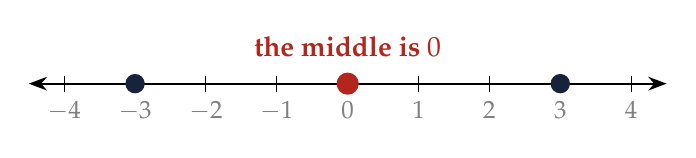
\begin{tikzpicture}[x=0.9cm]
\draw[thick,{Stealth}-{Stealth}] (-4.5,0)--(4.5,0);
\foreach \i in {-4,...,4} {\draw (\i,-0.1)--(\i,0.1); \node[below,gray] at (\i,-0.1){\small$\i$};}
\fill[fink] (-3,0) circle(3.5pt) (3,0) circle(3.5pt);
\onslide<2->{\fill[fred] (0,0) circle(4pt); \node[above=6pt,fred]{\bfseries the middle is $0$};}
\end{tikzpicture}
\par\bigskip
\onslide<3->{Add and halve:\quad $\dfrac{-3 + 3}{2} = 0$ \ {\color{fteal}\checkmark}}\qquad
\onslide<4->{Subtract:\quad $\dfrac{3 - (-3)}{2} = 3$ \ {\color{fred}$\times$}}\par\bigskip
\onslide<5->{\defn{\centering So the midpoint \key{adds} --- it's the \key{average} (mean).}}
\end{frame}

\begin{frame}{Midpoint formula}
\defn{\centering $M = \left(\dfrac{x_1 + x_2}{2},\ \dfrac{y_1 + y_2}{2}\right)$}\par\medskip
\begin{columns}[c]
\begin{column}{0.55\textwidth}
\onslide<2->{Example: $A(2, 3)$, $B(8, 7)$}\par\medskip
\onslide<3->{$x$: \ $\tfrac{2 + 8}{2} = 5$}\par\smallskip
\onslide<4->{$y$: \ $\tfrac{3 + 7}{2} = 5$}\par\medskip
\onslide<5->{$M = \ans{(5, 5)}$}
\end{column}
\begin{column}{0.42\textwidth}\centering
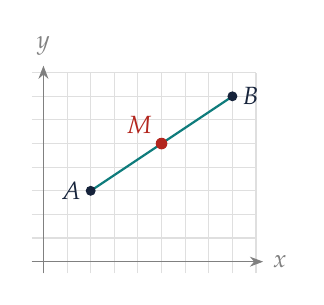
\begin{tikzpicture}[scale=0.3]
\grid{-0.5}{-0.5}{9}{8}
\onslide<2->{\draw[thick,fteal] (2,3)--(8,7);\fill[fink] (2,3) circle(6pt) node[left]{\small$A$} (8,7) circle(6pt) node[right]{\small$B$};}
\onslide<5->{\fill[fred] (5,5) circle(7pt) node[above left]{\small$M$};}
\end{tikzpicture}
\end{column}
\end{columns}
\end{frame}

\begin{frame}{Distance: simple case first}
\centering
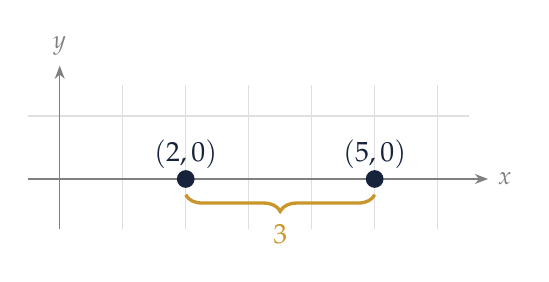
\begin{tikzpicture}[scale=0.8]
\grid{-0.5}{-0.8}{6.5}{1.5}
\fill[fink] (2,0) circle(4pt) node[above]{$(2, 0)$} (5,0) circle(4pt) node[above]{$(5, 0)$};
\onslide<2->{\draw[fgold,very thick,decorate,decoration={brace,amplitude=6pt,mirror}] (2,-0.25)--(5,-0.25) node[midway,below=7pt]{\bfseries $3$};}
\end{tikzpicture}
\par\bigskip
\onslide<3->{Count: $3$.\quad That's $5 - 2$ --- a \key{difference}.}
\end{frame}

\begin{frame}{Distance = Pythagoras on a grid}
\begin{columns}[c]
\begin{column}{0.44\textwidth}\centering
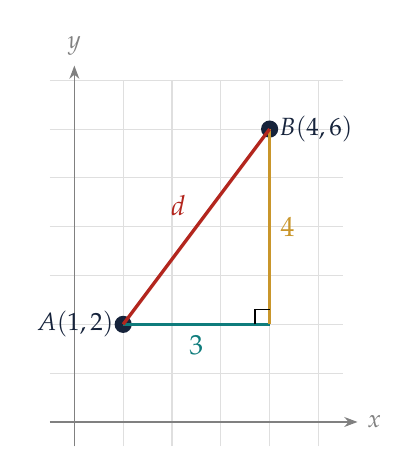
\begin{tikzpicture}[scale=0.62]
\grid{-0.5}{-0.5}{5.5}{7}
\fill[fink] (1,2) circle(5pt) node[left]{\small$A(1, 2)$} (4,6) circle(5pt) node[right]{\small$B(4, 6)$};
\onslide<2->{\draw[fteal,very thick] (1,2)--(4,2) node[midway,below]{$3$};\draw[fgold,very thick] (4,2)--(4,6) node[midway,right]{$4$};\draw (3.7,2)--(3.7,2.3)--(4,2.3);}
\onslide<3->{\draw[fred,very thick] (1,2)--(4,6) node[midway,above left]{$d$};}
\end{tikzpicture}
\end{column}
\begin{column}{0.54\textwidth}
Find $AB$.\par\medskip
\onslide<2->{Across $3$, up $4$.}\par\medskip
\onslide<3->{$d = \sqrt{3^2 + 4^2} = \sqrt{25} = \ans{5}$}\par\bigskip
\onslide<4->{\defn{\centering $d = \sqrt{(x_2 - x_1)^2 + (y_2 - y_1)^2}$}}
\end{column}
\end{columns}
\end{frame}

\begin{frame}{Two common mistakes}
\warn{Square \textbf{each} difference before adding: \ $\sqrt{3^2 + 4^2} = 5$, \ not $3 + 4 = 7$.}\par\bigskip\pause
\warn{Testing add vs.\ subtract? Don't use $0$ and $2$ --- both give $1$. Use $2$ and $4$: the middle is $3 = \frac{2 + 4}{2}$.}
\end{frame}

\begin{frame}{}
\begin{yourturn}
$P(-1, 4)$ and $Q(5, -4)$.\quad Find the midpoint of $\overline{PQ}$ and the length $PQ$.
\end{yourturn}
\pause\bigskip
$M = \left(\dfrac{-1 + 5}{2},\ \dfrac{4 + (-4)}{2}\right) = \ans{(2, 0)}$\par\medskip
\pause $PQ = \sqrt{(5 - (-1))^2 + (-4 - 4)^2} = \sqrt{6^2 + 8^2} = \sqrt{100} = \ans{10}$
\end{frame}

\closeframe{\begin{itemize}\setlength\itemsep{10pt}
\item \key{Midpoint = Mean}: add the coordinates, divide by 2.
\item \key{Distance = Difference}: subtract, square, add, square root.
\item The distance formula is just the Pythagorean Theorem.
\end{itemize}}
\end{document}
